% =====================================================================
%  chunks/ch03d.tex —— 原书 p.64–69（PDF 71–76）
%  第 3 章 §4 奇异同调、覆叠与层
% =====================================================================
% [原文 p.64]
（这里 $[\pi_1,\pi_1]$ 表示群 $\pi_1$ 的换位子群，即由那些在把 $\pi_1$ 交换化之后变为单位元的元素构成的子群。）作为这一命题的延伸，有 \emph{Hurewicz 定理}：

\emph{若 $\pi_i(K)=0$（$0<i<n$），则 $H_i(K;\Z)=0$（$0<i<n$）；又若 $n>1$，则存在自然同构}
\begin{equation}
  H_n(K;\Z)\cong\pi_n(K). \tag{3.19}
\end{equation}

（注意：对道路连通空间，相对于不同基点的同伦群彼此典范同构；因此今后不再明确标出基点，对相对同伦群 $\pi_i(K,L)$（$L$ 道路连通）也作同样处理。）

Hurewicz 定理的相对形式如下：\emph{若 $\pi_i(K,L)=0$（$0<i<n$），则 $H_i(K,L;\Z)=0$（$0<i<n$）；又若 $n>1$，则存在自然同构}
\begin{equation}
  H_n(K,L;\Z)\cong\pi_n(K,L)/\{a=t(a)\}, \tag{3.20}
\end{equation}
\emph{其中 $a$ 取遍 $\pi_n(K,L)$，$t$ 取遍 $\pi_1(L)$；后者看作按前面所定义的方式作用在 $\pi_n(K,L)$ 上的一组算子。}

这一相对化的 Hurewicz 定理其实更为完整，因为它在非单连通的情形下也适用，从而把 Hopf 定理包含在内。

\begin{example*}
设 $L$ 是 CW 复形 $K$ 的道路连通子复形，且 $K/L$ 是 $k$ 个 $n$ 维球面的花束，$n>1$：
\[
  K/L=S_1^n\vee\cdots\vee S_k^n,
\]
则 $\pi_n(K,L)$ 作为 $\Z[\pi]$-模（$\pi=\pi_1(L)$）是自由的，有 $k$ 个自然的自由生成元，依次对应花束中的各个球面。\hfill$\square$
\end{example*}

\section{单纯复形与其他同调论。奇异同调。覆叠与层。层的正合列与上同调}
\takeaway{本节用单形为任意拓扑空间构造奇异同调：奇异单形是标准单形到空间的映射，链复形按逐点方式定义，同伦不变性由此自动成立。随后引入以层为系数的上同调，并用覆叠空间的链复形把它化为可计算的形式。}

本节我们将用单形作工具，为任意拓扑空间 $X$ 构造一种同调论。我们还要定义系数取自层（sheaf）的上同调群；这在涉及复流形理论与复分析的各种问题中颇为重要。

我们从一般空间 $X$ 的「奇异」同调论讲起。所谓 $X$ 的一个 $n$ 维\emph{奇异单形}，是指一对 $(\sigma^n,f)$，其中 $\sigma^n$ 是标准 $n$-单形，$f$ 是该单形到 $X$ 的映射：

% [原文 p.65]
\[
  f\colon\sigma^n\longrightarrow X.
\]

$X$ 的奇异 $n$-单形于是（可以说）构成一族连续变化的映射 $f\colon\sigma^n\to X$。所谓 $X$ 中的一个\emph{奇异 $n$-链}，是指有限多个奇异单形的整系数线性组合。我们把相应的\emph{奇异链复形}记为 $C_*(X)$，其边缘算子 $\partial\colon C_n(X)\to C_{n-1}(X)$ 在奇异单形 $(\sigma^n,f)$ 上由下式定义：
\begin{equation}
  \partial(\sigma^n,f)=\sum_{j=0}^{n}(-1)^j\bigl(\sigma_j^{n-1},f\bigr), \tag{4.1}
\end{equation}
其中 $\sigma_j^{n-1}$ 是 $\sigma^n$ 的第 $j$ 个（定向的）$(n-1)$ 维面。借助奇异链复形 $C_*(X)$，按通常方式定义 $X$ 的\emph{奇异同调群}与\emph{奇异上同调群}。容易验证，它们是 $X$ 的同伦不变量，并且是函子的。同样容易看出，单点空间的奇异（上）同调群在非零维数上为零。向任意阿贝尔系数群 $G$ 的推广与前面基本相同。奇异相对同调群与上同调群 $H_j(X,A;G)$、$H^j(X,A;G)$ 完全类似地定义。若 $G$ 是环，则可类似地定义奇异上同调类的乘法，使奇异上同调群的直和 $H^*(X;G)$ 成为分次环，即\emph{$G$ 上的奇异上同调环}。最后还可以证明：若 $X$ 是单纯复形或 CW 复形，则奇异同调群与奇异上同调群同前面所定义的（上）同调群重合（即典范同构）。

奇异同调在考察从一个复形到另一个复形的映射空间时特别方便；更确切地说，在考察映射空间的同伦不变量时特别方便，而这些不变量对于建立计算球面及其他重要复形的同伦群所需的技术工具至关重要。

如前所述，对某几类拓扑空间，特别是复几何与复分析中出现的那些，以「层」为系数的上同调论是很有用的。

拓扑空间 $X$ 上的一个（群、环等的）\emph{预层}（presheaf）$\cF$ 是这样一种对应：它给 $X$ 的每个开集 $U$ 指定一个群（或环等）$\cF_U$，并给开集的每个包含关系 $V\subset U$ 指定一个同态
\begin{equation}
  \varphi_{VU}\colon\cF_U\longrightarrow\cF_V, \tag{4.2}
\end{equation}
称为相应于包含 $V\subset U$ 的\emph{限制同态}。此外还要求：若 $W\subset V\subset U$ 都是开集，则
\begin{equation}
  \varphi_{WV}\circ\varphi_{VU}=\varphi_{WU}. \tag{4.3}
\end{equation}
若预层还具有以下几条性质，就称为\emph{层}（sheaf）：

% [Tutor Note: 奇异同调的同伦不变性并非显然：通常的证明要先用重心重分（subdivision）把奇异链复形与单纯链复形在链同伦意义下等同起来，再引用单纯情形。初学者常误以为「单形连续形变」就能直接给出链同伦，实际上缺了重分这一步。]

% [原文 p.66]
(i) 对 $U$ 的任一由开集 $V_\alpha\subset U$ 构成的开覆盖 $\bigcup_\alpha V_\alpha=U$，若所有限制同态 $\varphi_{V_\alpha U}$ 在某个元素 $f\in\cF_U$ 上都为零，即 $\varphi_{V_\alpha U}(f)=0$，则应推出 $f=0$。

(ii) 给定如 (i) 中的开集 $V_\alpha$，并从每个 $\cF_{V_\alpha}$ 中各取一个元素 $f_\alpha$；若对任意的 $\alpha,\beta$，相应于包含 $W_{\alpha\beta}=V_\alpha\cap V_\beta\subset V_\alpha$ 与 $W_{\alpha\beta}\subset V_\beta$ 的两个限制同态彼此一致，即
\begin{equation}
  \varphi_{W_{\alpha\beta}V_\alpha}(f_\alpha)=\varphi_{W_{\alpha\beta}V_\beta}(f_\beta), \tag{4.4}
\end{equation}
则应存在元素 $f\in\cF_U$，使对一切 $\alpha$ 有
\[
  \varphi_{V_\alpha U}(f)=f_\alpha .
\]

群（或环等）$\cF_U$ 中定义在区域 $U\subset X$ 上的元素，称为层 $\cF$ 在 $U$ 上的\emph{截面}。

% [Tutor Note: 层公理的这两条容易读混：条件 (i) 说的是限制映射的分离性——局部全部为零则整体为零；条件 (ii) 说的是局部截面的粘合性——在各重叠处一致的局部截面必来自一个整体截面。把预层补成层的手续（层化）正是为满足这两条而设。]

\begin{example}{1}
\emph{常层}对每个开集 $U$ 都有 $\cF_U=G$，其中 $G$ 是某个固定的群（或环等）。
\end{example}

\begin{example}{2}
\emph{连续函数芽层}。这里每个 $\cF_U$ 是定义在 $U$ 上的实值函数环。类似地有光滑函数芽层；若取复值，则有全纯、亚纯或代数函数芽层，分别定义在光滑流形、复流形或代数簇 $X$ 上。更一般地，可考虑 $X$ 上某一光滑类别的向量场或一般张量场的芽层，甚至 $X$ 上任意纤维丛的截面的芽层（见下文）。
\end{example}

\begin{figure}[htbp]
  \centering
  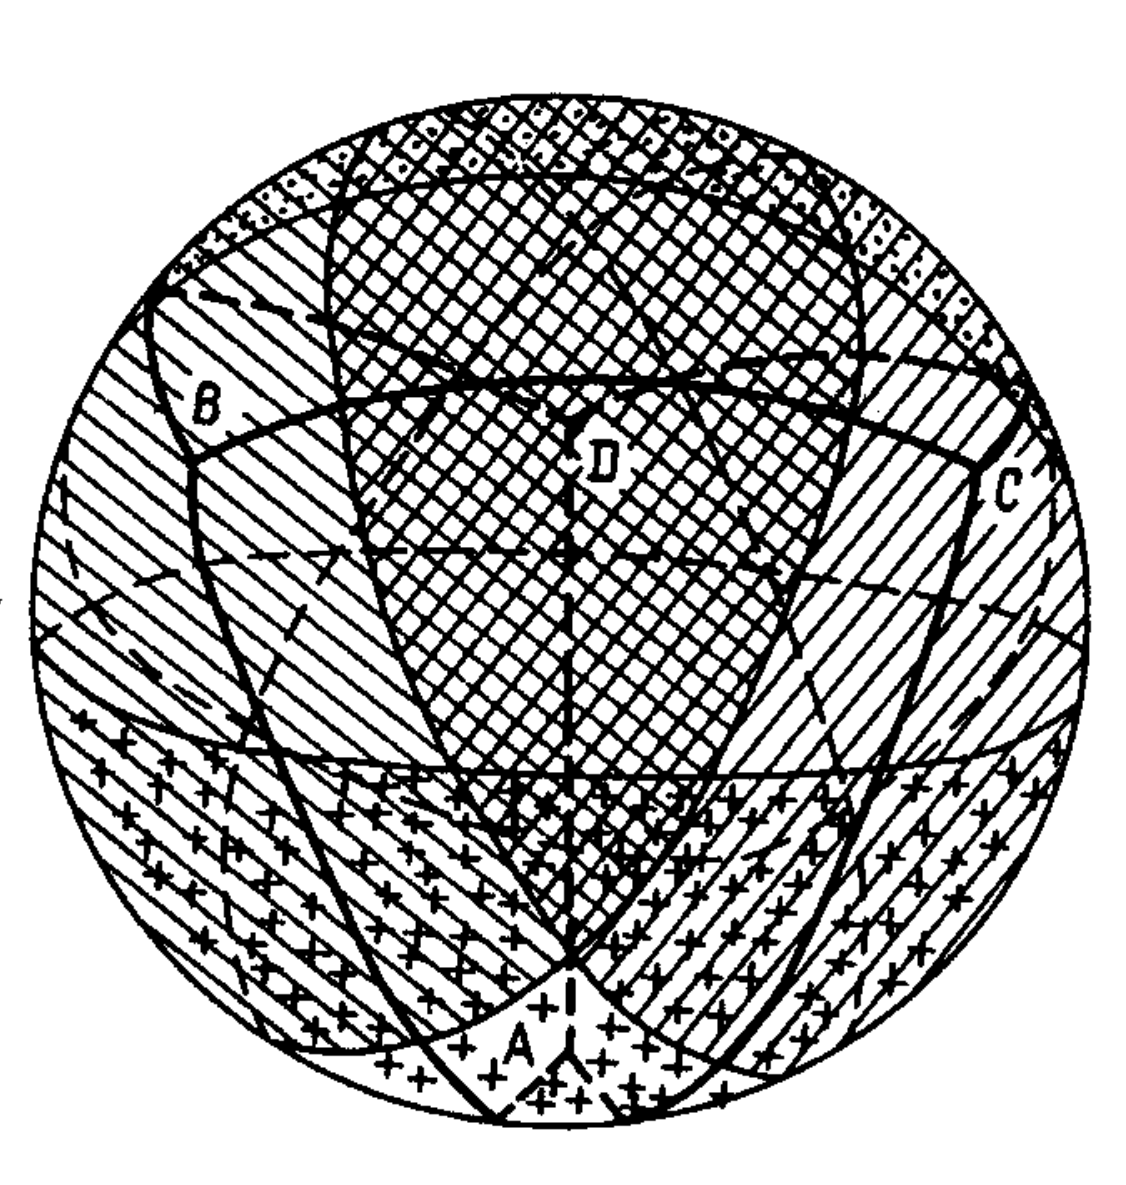
\includegraphics[width=0.42\textwidth]{figures/fig3_7.png}
  \figtitle{3.7}{此处的神经（nerve）是四面体 $ABCD$}
\end{figure}

20 世纪 20 年代，Lefschetz 开创了一个纲领：把组合拓扑的代数方法用于研究一般空间；其中的早期进展由 Vietoris、Alexandrov 和 Čech 作出。

% [原文 p.67]
Alexandrov 引入了由空间 $X$ 的可数多个开子集 $V_\alpha$ 构成的覆盖的\emph{神经}（nerve）概念，其中 $\bigcup_\alpha V_\alpha=X$；这就是如下定义的单纯复形 $K\{V_\alpha\}$：把 $\{V_\alpha\}$ 的指标 $\alpha_0,\alpha_1,\dots$ 取作 $K\{V_\alpha\}$ 的顶点，而把由 $n+1$ 个指标组成的有限子集 $\{\alpha_{i_0},\dots,\alpha_{i_n}\}$ 视为一个 $n$-单形，只要对应的开集有非空交（见图 3.7）：
\[
  V_{\alpha_{i_0}}\cap\cdots\cap V_{\alpha_{i_n}}\neq\varnothing .
\]

神经 $K=K\{V_\alpha\}$ 的上同调群 $H^j(K;G)$ 就称为覆盖 $\{V_\alpha\}$ 的\emph{上同调群}。若覆盖 $\{W_\kappa\}$「内接」（inscribed）于覆盖 $\{V_\alpha\}$，即每个 $W_\kappa$ 都含于某个 $V_\alpha$，则存在神经之间的自然单纯映射 $K\{W_\kappa\}\to K\{V_\alpha\}$——把 $K\{W_\kappa\}$ 的每个顶点 $\kappa$ 送到满足 $W_\kappa\subset V_\alpha$ 的任一顶点 $\alpha$（若这样的 $\alpha$ 不止一个，任取其一）。这一顶点映射确实决定一个单纯映射：因为若 $W_{\kappa_0}\cap\cdots\cap W_{\kappa_n}\neq\varnothing$，而 $W_{\kappa_j}\subset V_{\alpha_j}$，则交 $V_{\alpha_0}\cap\cdots\cap V_{\alpha_n}$ 也非空。于是有神经之间的单纯映射
\[
  \Psi_{WV}\colon K\{W_\kappa\}\longrightarrow K\{V_\alpha\}.
\]

还须注意，对空间 $X$ 的任意两个覆盖 $\{V_\alpha\}$ 与 $\{U_\beta\}$，总存在同时内接于这两个覆盖的覆盖 $\{W_\kappa\}$（例如取 $W_\kappa=U_\alpha\cap V_\beta$，$\kappa=\alpha\beta$），并有相应的神经映射：
% [Tutor Note: 原书 p.67 此处例中印作 $W_\kappa=U_\alpha\cap V_\beta$、$\kappa=\alpha\beta$，但涉及的覆盖是 $\{V_\alpha\}$ 与 $\{U_\beta\}$，按指标应对应 $U_\beta\cap V_\alpha$；此处照原书排印，读者按覆盖的指标理解即可。]
\[
\begin{array}{ccc}
  &                       & K\{V_\alpha\}\\
  & \nearrow_{\Psi_{WV}}  & \\
  K\{W_\kappa\} &         & \\
  & \searrow^{\Psi_{WU}}  & \\
  &                       & K\{U_\beta\}
\end{array}
\]
由此得到由复形 $K\{V_\alpha\}$ 及它们之间的单纯映射构成的\emph{逆系统}（inverse system，亦称「谱」）$\{K\{V_\alpha\},\Psi_{WV}\}$。可以把逆系统 $\{K\{V_\alpha\},\Psi_{WV}\}$ 看作空间 $X$ 的一个单纯逼近；例如当 $X$ 是紧致度量空间时，$\{K\{V_\alpha\},\Psi_{WV}\}$ 的逆极限同胚于 $X$。

每个单纯映射 $\Psi_{WV}\colon K\{W_\kappa\}\to K\{V_\alpha\}$ 诱导相应覆盖的上同调群之间的同态
\[
  \Psi^*_{WV}\colon H^j(K\{V_\alpha\};G)\longrightarrow H^j(K\{W_\kappa\};G),
\]
于是可以取由群与同态构成的系统 $\{H^j(K\{V_\alpha\};G),\Psi^*_{WV}\}$ 的\emph{直极限}，称为空间 $X$ 的第 $j$ 个\emph{谱（或 Čech）上同调群}。直极限的定义大致如下：

% [原文 p.68]
以所有覆盖 $\{V_\alpha\}$ 的 $H^j(K\{V_\alpha\};G)$ 中元素为生成元，把元素 $x\in H^j(K\{V_\alpha\};G)$ 与 $y\in H^j(K\{U_\beta\};G)$（它们可以属于不同的覆盖）看作相等——即把这一点作为元素间的阿贝尔群关系强加下去——只要存在更细的覆盖 $\{W_\kappa\}$，使这两个元素在群 $H^j(K\{W_\kappa\};G)$ 中的像 $\Psi^*_{WV}(x)$ 与 $\Psi^*_{WU}(y)$ 重合：
\[
\begin{array}{ccc}
  & & H^j(K\{V_\alpha\};G)\\
  & \swarrow_{\Psi^*_{WV}} & \\
  H^j(K\{W_\kappa\};G) & & \\
  & \nwarrow^{\Psi^*_{WU}} & \\
  & & H^j(K\{U_\beta\};G)
\end{array}
\]

空间 $X$ 的第 $j$ 个\emph{谱（或 Čech）同调群}类似地定义为 $X$ 的所有覆盖的第 $j$ 个同调群的逆极限，当然此时所有同态的方向都反过来。谱上同调与谱同调论的现代表述归功于 Čech。

给定任一已三角剖分的流形，构造一个其同调群与上同调群同原三角剖分一致的开覆盖并不困难。（做法是：取该流形足够细的三角剖分 $K$，注意 Poincaré 对偶复形 $DK$ 给出一个由开凸多胞形 $U_\alpha=\operatorname{Int}D\sigma^0_\alpha$ 构成的覆盖，其中 $\sigma^0_\alpha$ 是三角剖分 $K$ 的顶点。此时可以看出，这个覆盖的神经 $K\{U_\alpha\}$ 与复形 $K$ 的重心重分相合。）于是借助单纯同调在重心重分之下的不变性，就得到 Čech 同调与单纯同调版本的等价。由于 Čech 同调群显然在同胚下不变，由此便得到单纯同调群在同胚下的不变性（而不是它们的同伦不变性）。

利用拓扑空间 $X$ 的覆盖的神经，可以给出 $X$ 的以 $X$ 上层 $\cF$ 为系数的上同调群的自然定义；这一概念最初似乎是由 Leray 引入的。设 $K\{V_\alpha\}$ 是 $X$ 的覆盖 $\{V_\alpha\}$ 的如上定义的神经。给神经的每个单形 $(\alpha_0,\dots,\alpha_n)$ 配上显然的群（或环等）：
\[
  (\alpha_0,\dots,\alpha_n)\longrightarrow\cF_{V_{\alpha_0}\cap\cdots\cap V_{\alpha_n}} .
\]

取值于层 $\cF$ 的上链 $f$（对应于覆盖 $\{V_\alpha\}$）就定义为 $K\{V_\alpha\}$ 的单形上的这样一类函数：它在任意单形 $(\alpha_0,\dots,\alpha_n)$ 处的值属于 $\cF_{V_{\alpha_0}\cap\cdots\cap V_{\alpha_n}}$。上边缘算子 $\partial^*$ 自然地定义为

% [Tutor Note: Čech 上同调取直极限，而 Čech 同调取逆极限，两者并不对称：逆极限一般不与商交换，可能丢掉信息。这正是后来层论上同调（导出函子）取代 Čech 同调的原因；在紧致度量空间等良好情形下，Čech 上同调与奇异上同调一致。]

% [原文 p.69]
\[
  \bigl(\partial^*f;(\alpha_0,\dots,\alpha_{n+1})\bigr)=\sum_{j=0}^{n+1}(-1)^j\varphi_j f(\alpha_0,\dots,\widehat{\alpha}_j,\dots,\alpha_{n+1}),
\]
其中 $\varphi_j$ 是限制同态
\[
  \varphi_j\colon\cF_{\bigl(\bigcap_{i\neq j}V_{\alpha_i}\bigr)}\longrightarrow\cF_{\bigl(\bigcap_i V_{\alpha_i}\bigr)} .
\]

由此得到对应于特定覆盖 $\{V_\alpha\}$ 的 $n$ 维层上同调群；而 $X$ 的以层 $\cF$ 为系数的上同调群 $H^n(X;\cF)$（即 $X$ 的第 $n$ 个上同调群）则是所有这些覆盖所产生的群构成的谱的极限。

% [Tutor Note: 这里的「谱的极限」是直极限而非逆极限：覆盖越细，可用的上链越多，群越大，故沿内接映射取直极限。原书下方按生成元与关系的语言重述，正是直极限的标准构造；与 p.68 末对 Čech 同调取逆极限恰成对照。]

\begin{example}{1}
对光滑流形 $M^n$ 上连续函数的芽层 $\cF$，或光滑类 $C^k$（$1\le k\le\infty$）函数的芽层，不难证明
\[
  H^j(M^n;\cF)=0,\qquad j>0 .
\]
这里的零阶上同调群 $H^0(M^n;\cF)$ 正是定义在整个流形 $M^n$ 上的（容许）函数构成的无穷维空间。
\end{example}

\begin{example}{2}
对闭复流形 $X$ 上全纯函数的芽层 $\cF$，有：
\begin{itemize}
  \item[(i)] $H^0(X;\cF)\cong\C$（因为整体全纯函数只有常函数）；
  \item[(ii)] 当 $j>0$ 时，$H^j(X;\cF)$ 是有限维向量空间。
\end{itemize}
\end{example}

子层 $\cF_1\subset\cF_2$ 与商层 $\cF_3=\cF_2/\cF_1$ 可按自然方式定义；不过定义商时可能出现困难，所以实际上商一般只能作为预层来定义。于是有层的短正合列：
\[
  0\longrightarrow\cF_1\xrightarrow{i}\cF_2\xrightarrow{j}\cF_3\longrightarrow 0 .
\]
由此得到如下的层上同调正合列，它的特例涵盖了（上）同调正合列的各种形式：
\begin{equation}
  \cdots\longrightarrow H^q(X;\cF_1)\xrightarrow{i^*}H^q(X;\cF_2)\xrightarrow{j^*}H^q(X;\cF_3)\xrightarrow{\partial^*}H^{q+1}(X;\cF_1)\longrightarrow\cdots . \tag{4.5}
\end{equation}

% [Tutor Note: 商层 $\cF_2/\cF_1$ 一般不是层而只是预层——逐点取商得到的截面对局部化不封闭；须再作层化才得到层。原书此处特意点明这一点，读 (4.5) 时须记住其中的 $\cF_3$ 已是层化后的层，否则短正合列在层范畴中未必成立。]

\begin{example}{1}
设 $\cF_2$ 是 CW 复形 $K$ 上的常层，即给 $K$ 的每个开集配上某个固定群 $G$。取 $\cF_2$ 的子层 $\cF_1$ 为：在 $K$ 的给定子复形 $L$ 上为常层（$=G$），在 $L$ 之外为零。于是 $K$ 的取值于 $\cF_2$ 的第 $q$ 个上同调群就是 $H^q(K;G)$，取值于 $\cF_1$ 的是 $H^q(L;G)$。正合列 (4.5) 化为对 $(K,L)$ 的上同调正合列（见 §3 的 (3.4)）。
\end{example}

% CHUNK ch03d DONE
